\section{系统设计}

\subsection{系统总体功能设计}

本系统的整体架构采用Django的MVT三层设计模式,其中M表示Model层、V表示View层以及T表示Template层。从工厂信息管理着手,如图\ref{fig:sysarc}所示,首先对系统总体功能进行设计,选择开发环境以及数据库,之后对数据层进行功能设计,例如事务管理以及读写数据库等,然后设计业务层的业务逻辑,例如交易信息管理、员工信息管理和人脸识别签到等,之后使用模板渲染对前端页面进行后端数据的渲染,最后向用户展示,系统的总体功能模块如图\ref{fig:funmod}所示。

\begin{figure}[H]
    \centering
    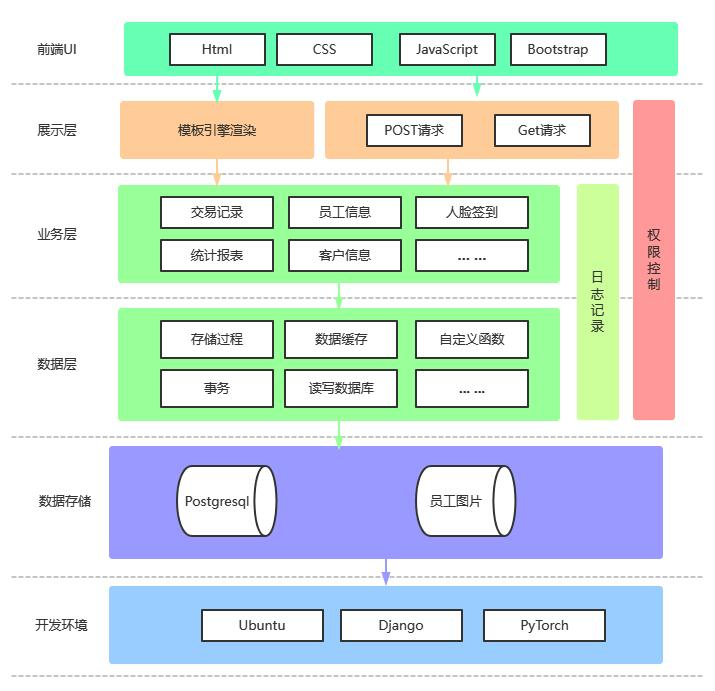
\includegraphics[width=.65\textwidth]{figures/4total.jpg}
    \caption{系统架构图}
    \label{fig:sysarc}
\end{figure}

\begin{figure}[H]
    \centering
    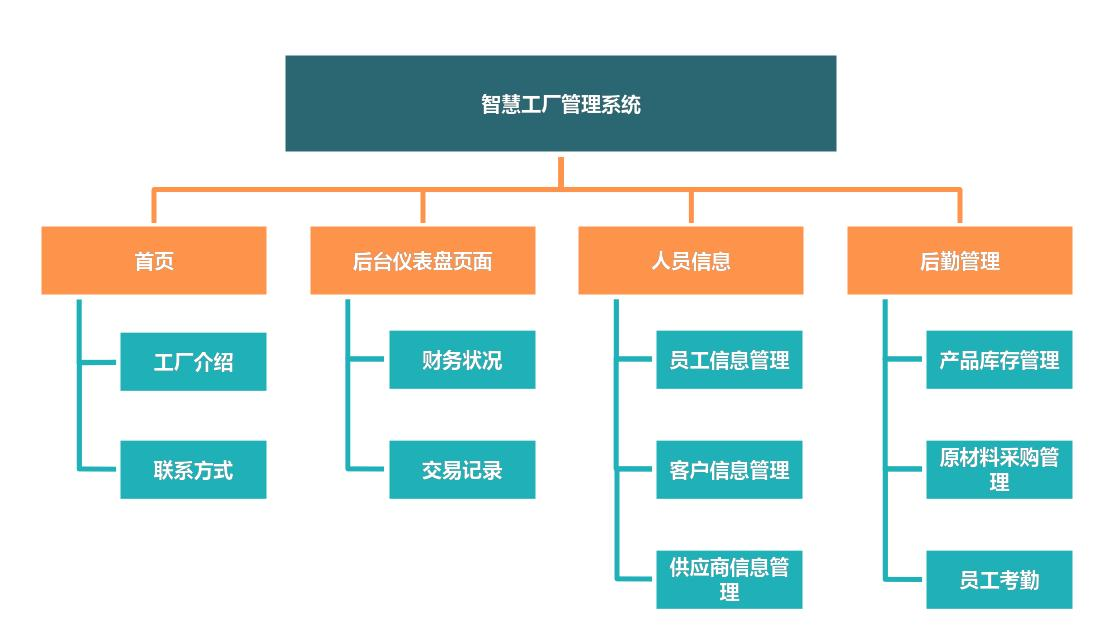
\includegraphics[width=.65\textwidth]{figures/4funmod.jpg}
    \caption{总体功能模块图}
    \label{fig:funmod}
\end{figure}

% \subsection{后台仪表盘页面设计}

% 在管理员输入正确的用户密码之后,进入到管理后台页面,向管理员展示当前工厂的运营情况的仪表盘面板总览,例如当前财务状况,月度的收入、支出以及利润,绘制年度收益概览折线图以及绘制月度收入概览饼图,在下方,向管理员展示最近的入账、出账交易记录。

\subsection{数据库设计}

在工厂管理中,首先要对三种不同的实体人物进行抽象,有员工信息、客户信息以及供应商信息。分别对三种实体信息进行抽象抽取,设计数据库关系,如表\ref{tab:emp}所示,给出了员工信息的关系表。

\begin{table}[H]
    \centering
    \zihao{5}
    \caption{员工信息设计表}
    \label{tab:emp}
    \begin{tabular}{cccc}
        \toprule
        字段名 & 数据类型 & 默认值 & 描述信息 \\
        \midrule
        name & CharField & NULL & 员工姓名 \\
        basicSalary & DecimalField & 0 & 基本工资 \\
        bonus & DecimalField & 0 & 奖金 \\
        total & DecimalField & 0 & 工资共计 \\
        isPaid & BooleanField & False & 是否支付薪资 \\
        lastSalary & DateField & NULL & 最后一次工资更新日期 \\
        designation & CharField & 其他 & 职称 \\
        address & CharField & NULL & 员工地址 \\
        phone & CharField & NULL & 电话号码 \\
        dob & DateField & NULL & 出生日期 \\
        doj & DateField & NULL & 入职日期 \\
        gender & IntegerField & 2 & 性别 \\
        \bottomrule
    \end{tabular}
\end{table}

对后勤信息管理部分进行抽象设计,有产品信息、原材料信息以及员工考勤的签到表。分别对产品和原材料的实体信息进行抽象并设计数据库关系表,如表\ref{tab:product}所示,给出了产品信息的关系表。

\begin{table}[H]
    \centering
    \zihao{5}
    \caption{产品信息设计表}
    \label{tab:product}
    \begin{tabular}{cccc}
        \toprule
        字段名 & 数据类型 & 默认值 & 描述信息 \\
        \midrule
        name & CharField & NULL & 产品名称 \\
        cost & DecimalField & NULL & 产品成本 \\
        wages & DecimalField & NULL & 产品利润 \\
        weight & DecimalField & NULL& 产品重量 \\
        \bottomrule
    \end{tabular}
\end{table}

之后将所有独立的实体表进行定义基数关系,其中包含在客户对某个产品进行下单时,定义客户表和产品表之间的多对多关系的订单表;在员工生产某一个产品时就会有多对多关系的工作表;供应商对某一种原材料进行供应时的多对多的供应表等,如图\ref{fig:er}所示,展示本系统关键实体的的E-R关系图。

\begin{figure}[H]
    \centering
    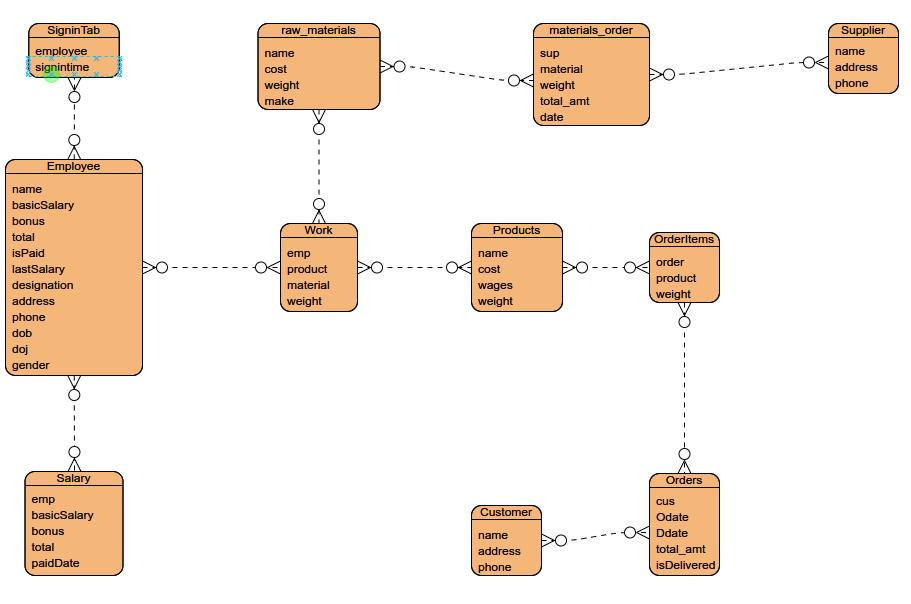
\includegraphics[width=.75\textwidth]{figures/4er.jpg}
    \caption{系统关键实体E-R图}
    \label{fig:er}
\end{figure}

\subsection{员工考勤功能设计}

本系统结合深度学习人脸识别技术,使用Facenet网络模型进行训练,来实现对员工考勤签到功能。进入到员工考勤页面,首先向管理员展示最近的员工签到表,包含员工姓名以及签到时间。进行人脸签到时,计算人脸图像的embedding编码,与本地员工人脸图像数据库进行比对,得到两者最小距离的员工,并且检查是否小于阈值,通过后便向签到表添加记录。

\subsubsection{构造数据集}

由于新冠疫情的影响,人们在日常出行的时候佩戴口罩是必不可少的。由于佩戴口罩对人脸进行了遮挡,所以在一些基于人脸识别的传统系统受到了很多挑战。所以本系统选择基于用于训练人脸识别的CASIA-Webface的人脸数据集基础之上,使用MaskTheFace工具对数据集进行构造,构造一个模拟佩戴口罩人脸数据集用于训练。CASIA-Webface由10,575位人物共494,414张人脸图像构成,部分人脸图像如图\ref{fig:webface}所示。

\begin{figure}[H]
    \centering
    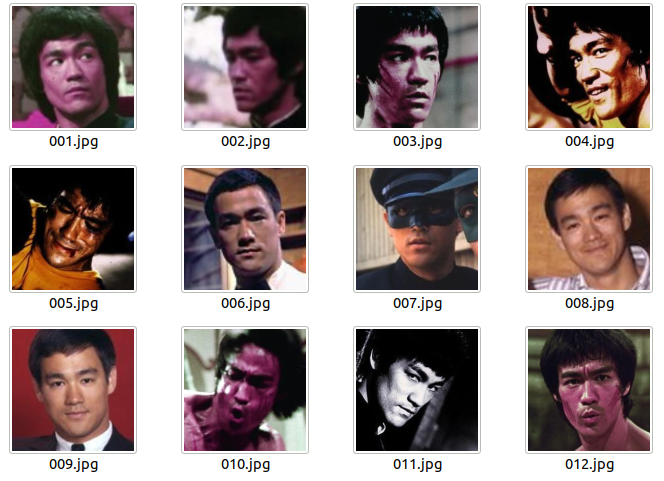
\includegraphics[width=.4\textwidth]{figures/4webface.png}
    \caption{CASIA-Webface人脸数据集部分图像}
    \label{fig:webface}
\end{figure}

训练完神经网络模型之后,使用LFW数据集和MFR2数据集进行测试评估模型的性能,参考模型对人脸识别的准确率。其中LFW是现实世界的涵盖各种自然可变因素的人脸数据集,由5,749位人物共13,233张人脸图像,其中1,680位人物有2张以上的人脸图像,部分人脸图像如图\ref{fig:lfw}所示。MFR2是现实世界的佩戴口罩的人脸数据集,由53位名人和政治家共269张佩戴口罩的人脸图像构成,部分人脸图像如图\ref{fig:mfr2}所示。

\begin{figure}[H]
    \centering
    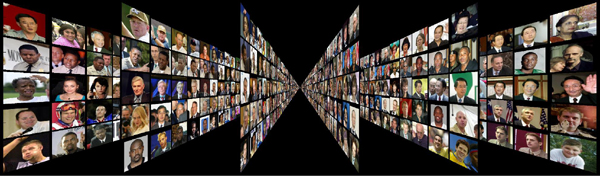
\includegraphics[width=.75\textwidth]{figures/4lfw.jpg}
    \caption{LFW人脸数据集部分图像}
    \label{fig:lfw}
\end{figure}

\begin{figure}[H]
    \centering
    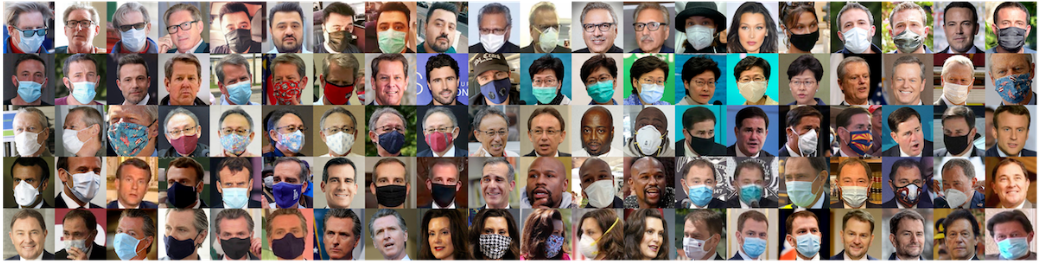
\includegraphics[width=.75\textwidth]{figures/4mfr2.png}
    \caption{MFR2人脸数据集部分图像}
    \label{fig:mfr2}
\end{figure}

\subsubsection{模型设计}

本系统选用Facenet网络模型用于人脸识别,模型整体结构如图\ref{fig:modelarc}所示,其中最左边表示一个批量的图像输入到深度卷积神经网络中,对卷积神经网络的输出进行$L_{2}$ normalization得到人脸图像的embedding编码,之后使用TripletLoss为损失函数进行训练。

\begin{figure}[H]
    \centering
    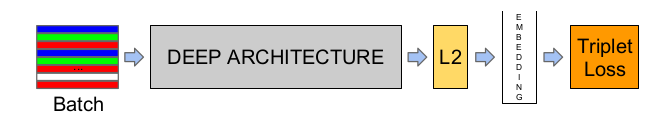
\includegraphics[width=.75\textwidth]{figures/4modelarc.png}
    \caption{模型整体架构图}
    \label{fig:modelarc}
\end{figure}

TripletLoss可以直接反映出人脸验证、识别和聚类所能达到的效果。换句话说,对于一张输入人脸图像$x$映射到特征空间$\mathbb{R}^d$中,通过$f(x)$得到embedding,来使得相同人物的人脸图像之间的平方距离更小(与成像条件相独立),而对于来自于不同人物的图像对之间的平方距离尽可能地大。

\subsubsection{TripletLoss损失函数}

人脸图像的embedding编码由$f(x)\in\mathbb{R}^d$表示,它将一张图像$x$嵌入到一个d维的欧式空间。并且将embedding编码限制到一个d维的超球面,也就是使得$\left \| f(x) \right \| _2=1$。在本模型中,要确保一个特定人物的图像$x_i^a$(anchor)尽可能接近与其相同人物的其它图像$x_i^p$(positive),而与剩余任何一个其他人物的图像$x_i^n$(negative)尽可能远,以上过程如图\ref{fig:tpltll}所示。

\begin{figure}[H]
    \centering
    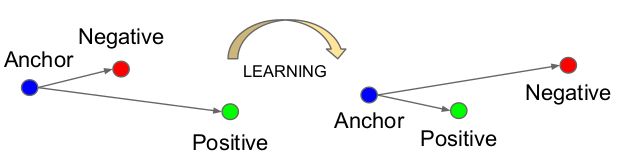
\includegraphics[width=.75\textwidth]{figures/4tpltll.png}
    \caption{TripletLoss训练图}
    \label{fig:tpltll}
\end{figure}

以上过程可以由公式\ref{eq:tpltll}表示,其中,$\alpha$表示正类图像对与负类图像对之间的边距,$\mathcal{T}$表示在训练集中所有可能的三元组集合。

\begin{equation}
    \left\|x_{i}^{a}-x_{i}^{p}\right\|_{2}^{2}+\alpha<\left\|x_{i}^{a}-x_{i}^{n}\right\|_{2}^{2}, \forall\left(x_{i}^{a}, x_{i}^{p}, x_{i}^{n}\right) \in \mathcal{T}
    \label{eq:tpltll}
\end{equation}

由此便可得到要被最小化的损失函数$L$,由公式\ref{eq:loss}表示。

\begin{equation}
    L=\sum_{i}^{N}\left[\left\|f\left(x_{i}^{a}\right)-f\left(x_{i}^{p}\right)\right\|_{2}^{2}-\left\|f\left(x_{i}^{a}\right)-f\left(x_{i}^{n}\right)\right\|_{2}^{2}+\alpha\right]_{+}
    \label{eq:loss}
\end{equation}

\subsubsection{模型评估性能指标}

所有的相同人物的人脸图像对$(i,j)$被表示为$\mathcal{P}_{\text {same}}$,不同人物的人脸图像对表示为$\mathcal{P}_{\text {diff}}$。之后,定义所有true accept的集合,由公式\ref{eq:ta}表示有人脸对$(i,j)$被正确地分为同一位人物,其中$D\left(x_{i}, x_{j}\right)$表示为一对图像之间的距离,$d$表示为距离阈值。

\begin{equation}
    \mathrm{TA}(d)=\left\{(i, j) \in \mathcal{P}_{\text {same }}, \text { with } D\left(x_{i}, x_{j}\right) \leq d\right\}
    \label{eq:ta}
\end{equation}

相似地,可以定义false accept,公式为\ref{eq:fa}。

\begin{equation}
    \mathrm{FA}(d)=\left\{(i, j) \in \mathcal{P}_{\text {diff }}, \text { with } D\left(x_{i}, x_{j}\right) \leq d\right\}
    \label{eq:fa}
\end{equation}

对于一个给定的人脸距离阈值$d$,验证率(validation rate)$VAL(d)$和错误接受率(false accept rate)$FAR(d)$被定义为公式\ref{eq:valfar}所示。

\begin{equation}
    \operatorname{VAL}(d)=\frac{|\mathrm{TA}(d)|}{\left|\mathcal{P}_{\text {same }}\right|}, \quad \operatorname{FAR}(d)=\frac{|\mathrm{FA}(d)|}{\left|\mathcal{P}_{\text {diff }}\right|}
    \label{eq:valfar}
\end{equation}